\appendix{}

\chapter{Supplemental Material for Chapter \ref{chap:Title of first chapter}}

%%%%%%%%%%%%%%%%%%%%%%%%%%%%%%%%%%%%%%%%%%%%%%%%%%%%%%%%%%%%%%%%%%%%%%%%%%%%%%%%
\section{Section name}
%%%%%%%%%%%%%%%%%%%%%%%%%%%%%%%%%%%%%%%%%%%%%%%%%%%%%%%%%%%%%%%%%%%%%%%%%%%%%%%%

\subsection{Subsection name}
Text here.

%%%%%%%%%%%%%%%%%%%%%%%%%%%%%%%%%%%%%%%%%%%%%%%%%%%%%%%%%%%%%%%%%%%%%%%%%%%%%%%%
\section{Supplementary Table Captions}
%%%%%%%%%%%%%%%%%%%%%%%%%%%%%%%%%%%%%%%%%%%%%%%%%%%%%%%%%%%%%%%%%%%%%%%%%%%%%%%%

The Supplemental Table can be found on the GitHub repository for this study labeled as \verb|SupplementaryTable.xlsx| at the following location: 

\noindent \href{https://github.com/Github/RepoName/}{\texttt{https://github.com/Github/RepoName/}}.

\par\noindent\dotfill

\subsubsection{Supplementary Table S1: Table title}
Text here.

%%%%%%%%%%%%%%%%%%%%%%%%%%%%%%%%%%%%%%%%%%%%%%%%%%%%%%%%%%%%%%%%%%%%%%%%%%%%%%%%
\section{Supplementary Figures}
%%%%%%%%%%%%%%%%%%%%%%%%%%%%%%%%%%%%%%%%%%%%%%%%%%%%%%%%%%%%%%%%%%%%%%%%%%%%%%%%

\begin{figure}[h]
    \centering
    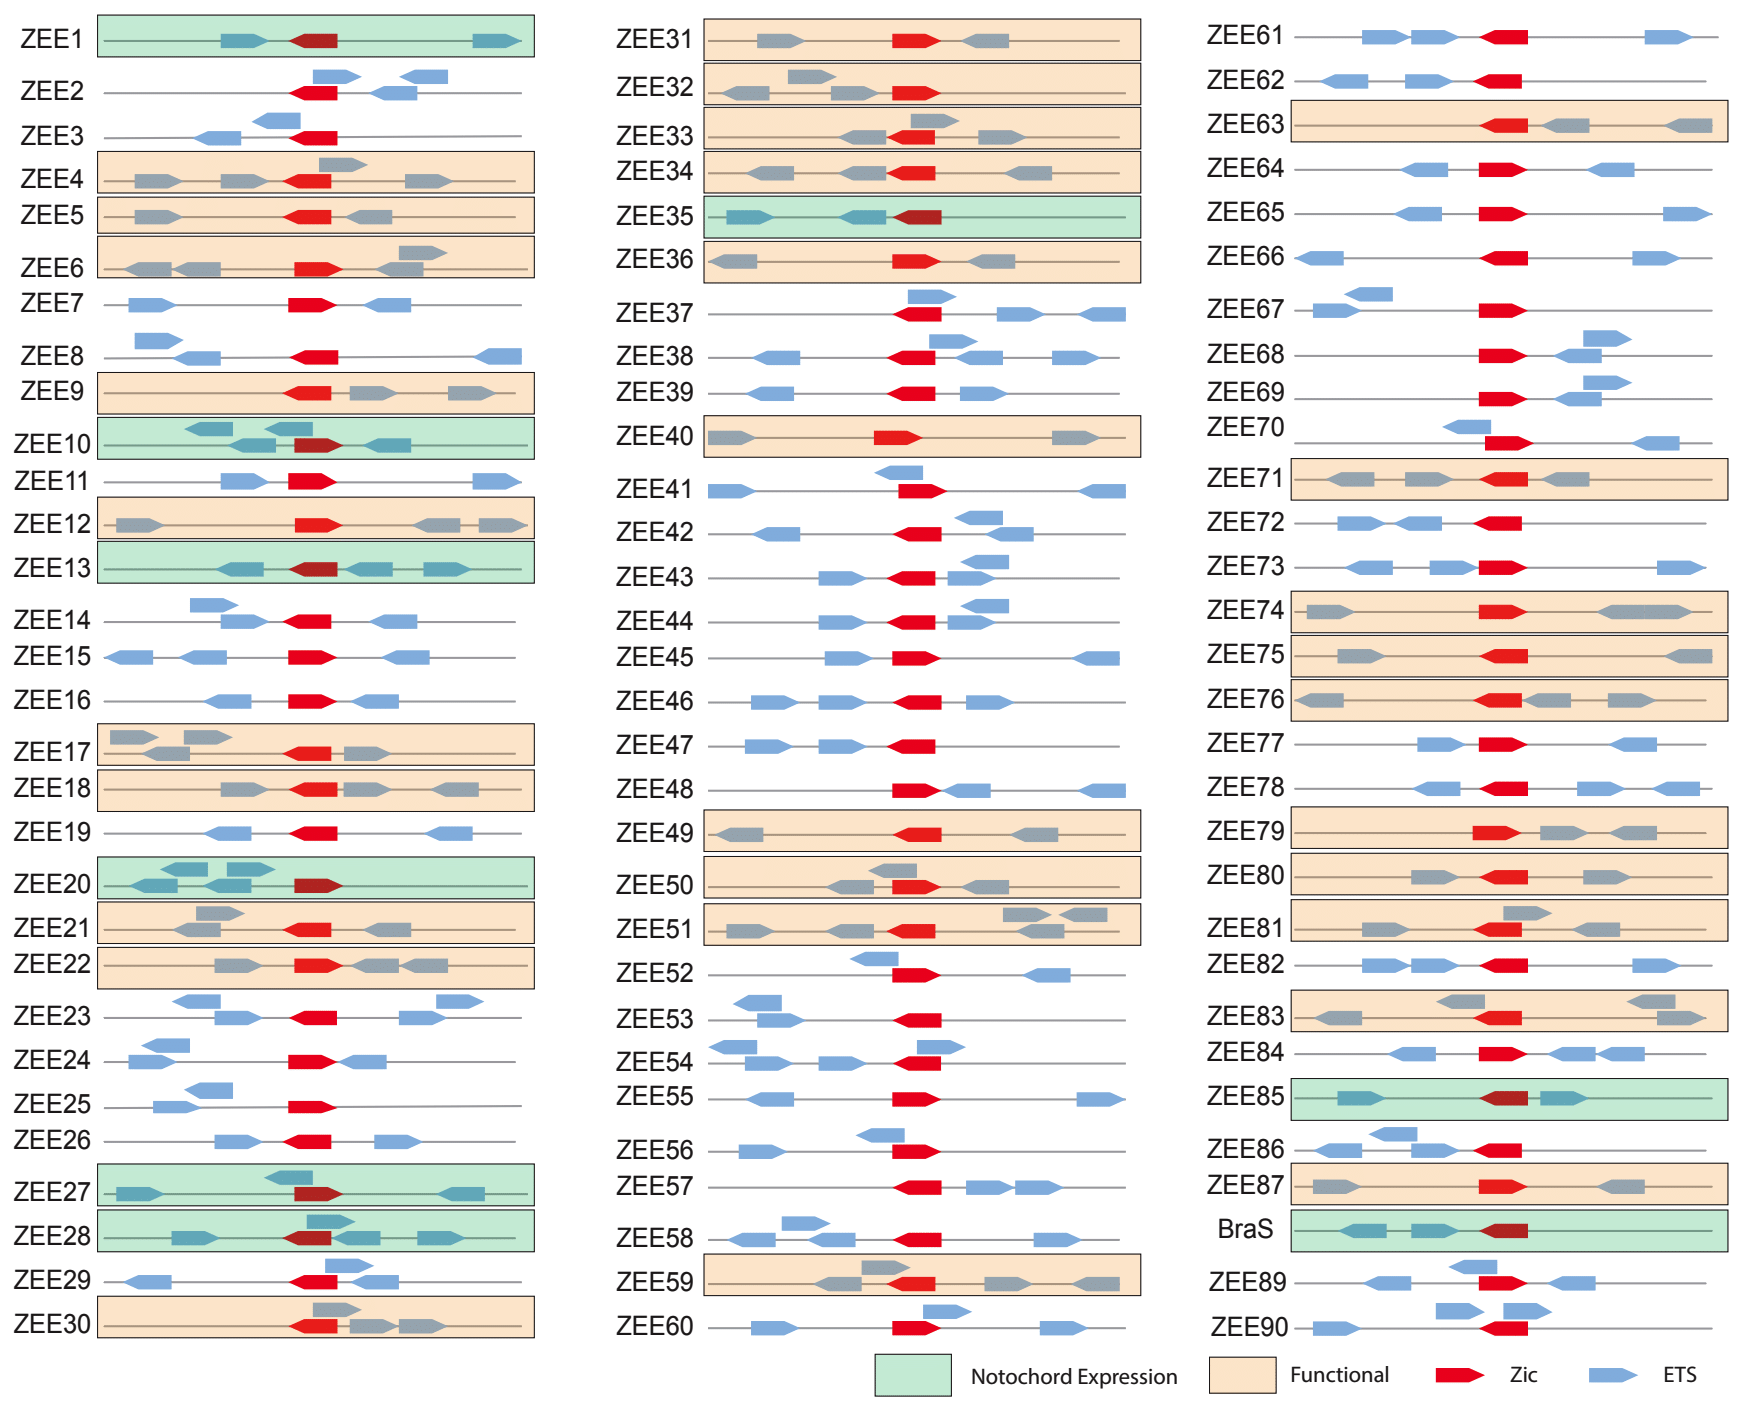
\includegraphics[scale=.2]{1_figures-and-files/FigS1_ZEE-Library.png}
    \caption[Figure title]{\textbf{Figure title.} Text here.}
    \label{fig:supplement tag for table of contents}
\end{figure}


%%%%%%%%%%%% Example of a split figure.
\begin{figure}[p]
    \centering
    \caption[Figure title]{Text here (\textit{Continued on next page.})}
    \label{fig:supplement tag2 for table of contents}
\end{figure}

\addtocounter{figure}{-1}

\captionsetup[figure]{list=no}
\begin{figure}[p]
    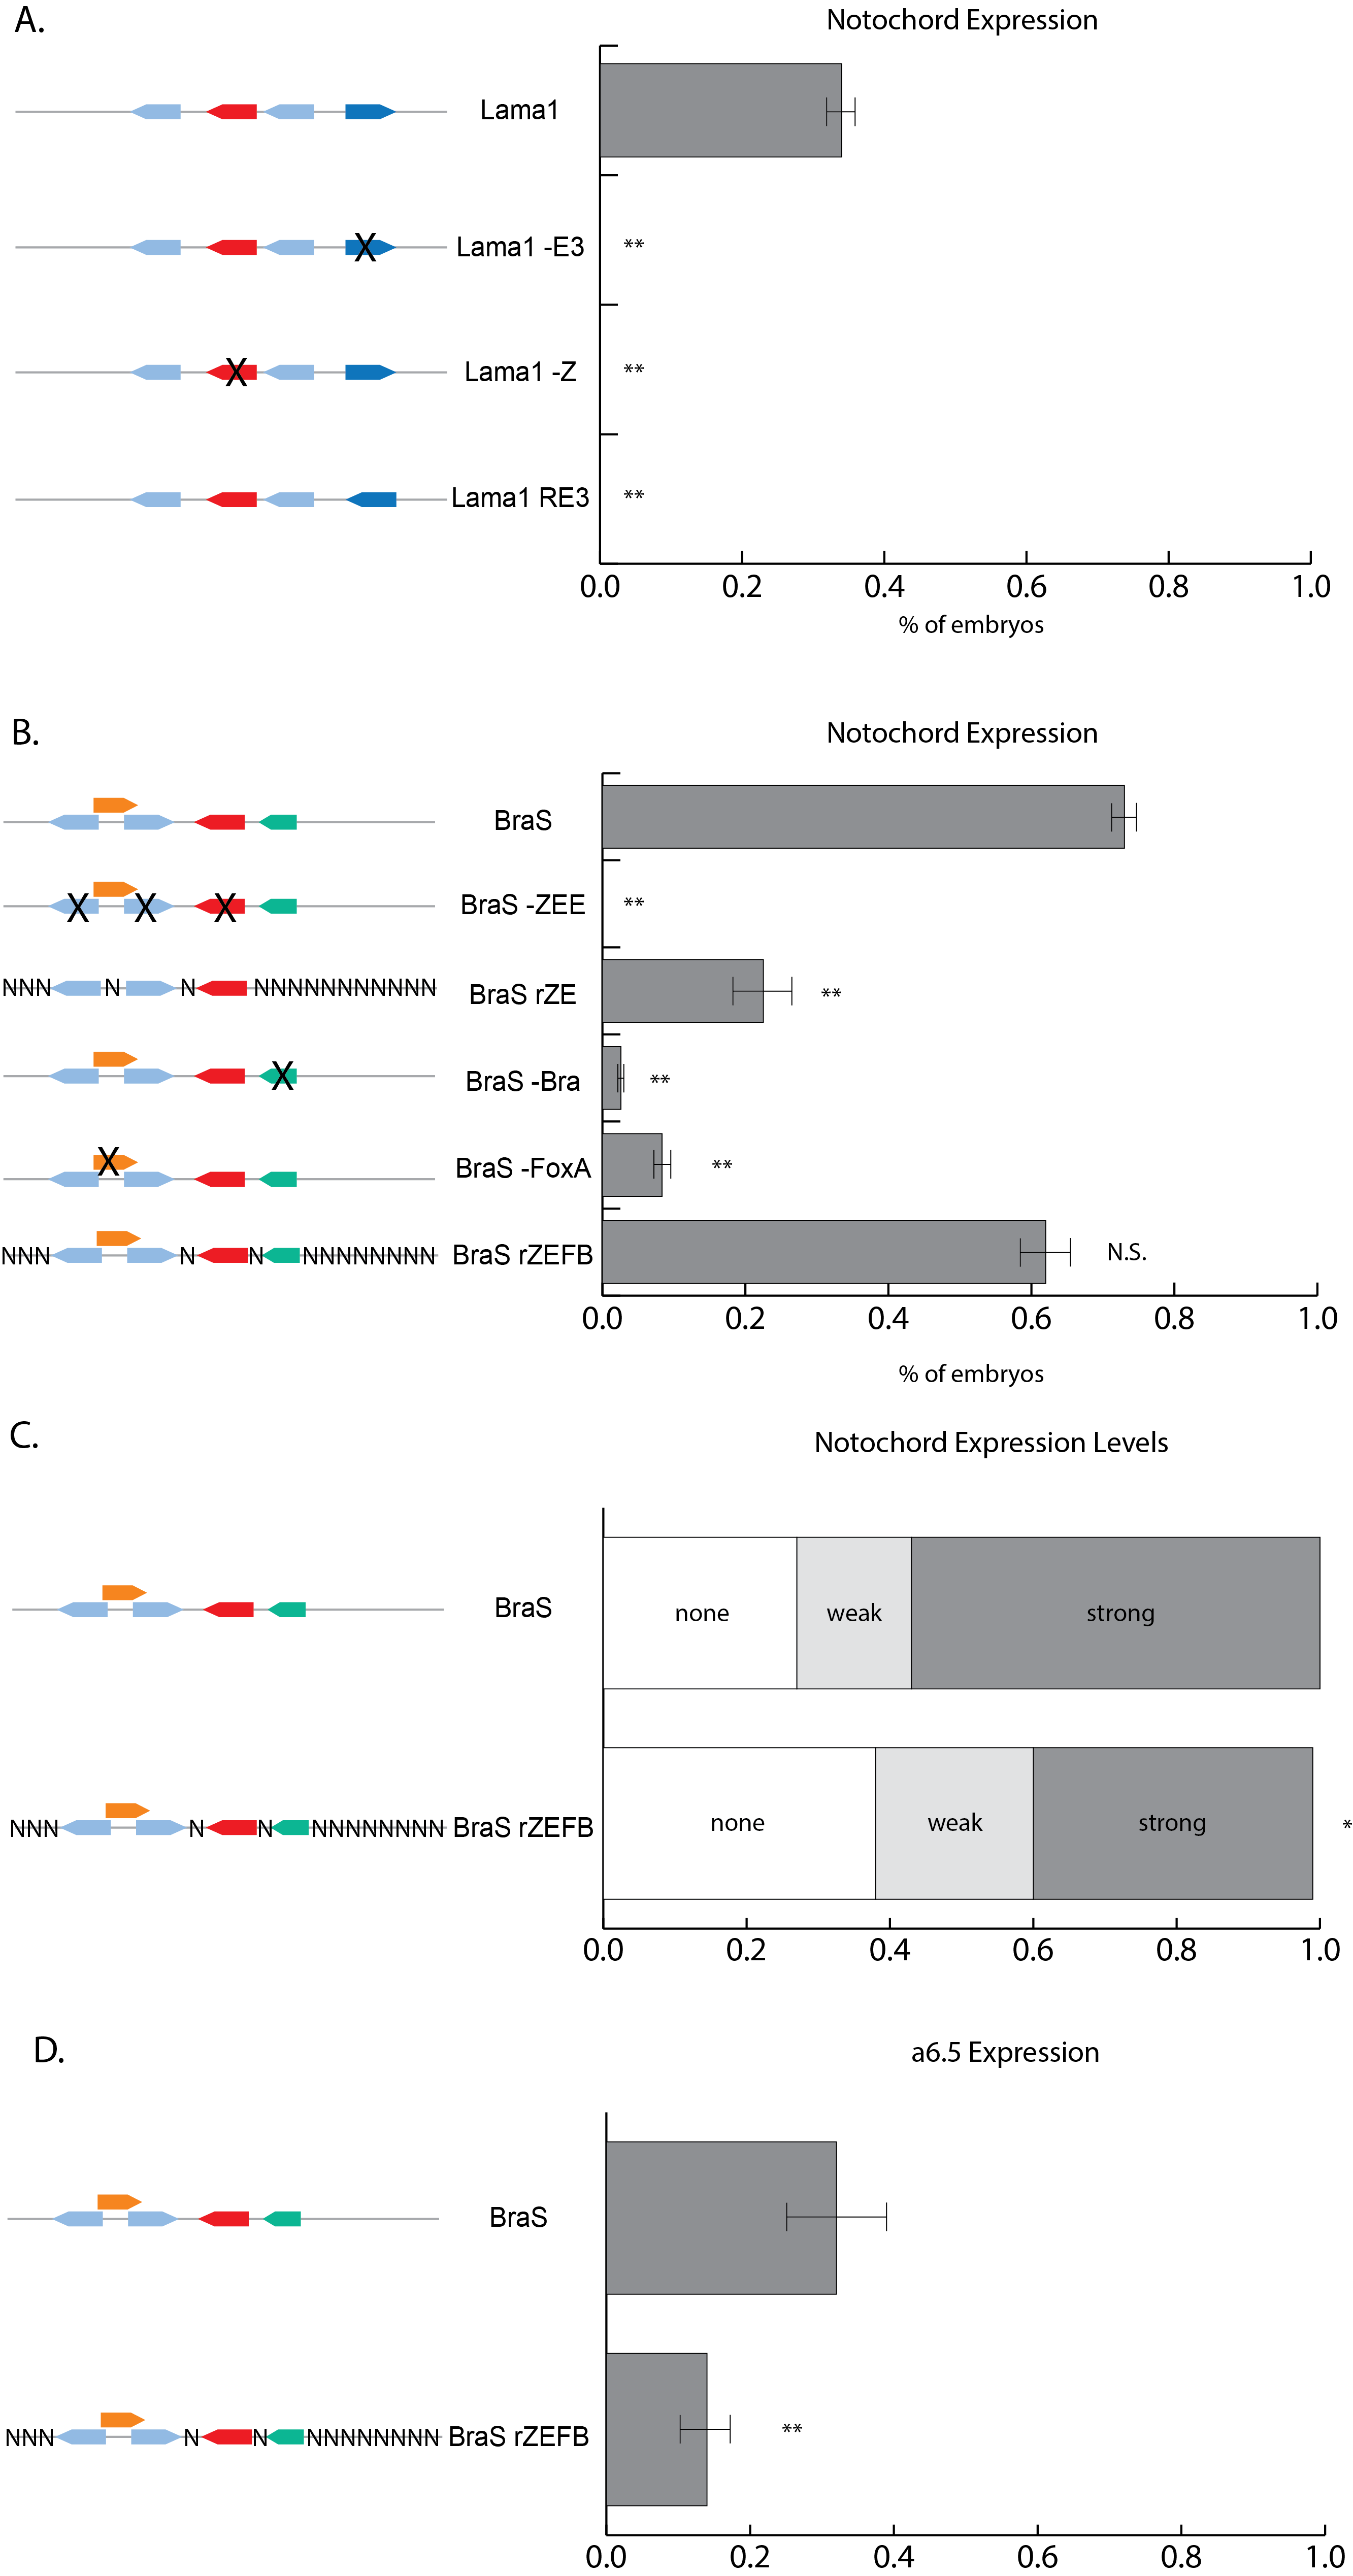
\includegraphics[scale=.5]{1_figures-and-files/FigS5_Notochord-Counting.png}
    \caption{(\textit{Continued from previous page.})}
\end{figure}
\captionsetup[figure]{list=yes}
%%%%%%%%%%%%